
\begin{figure}[t!]
    \centering
    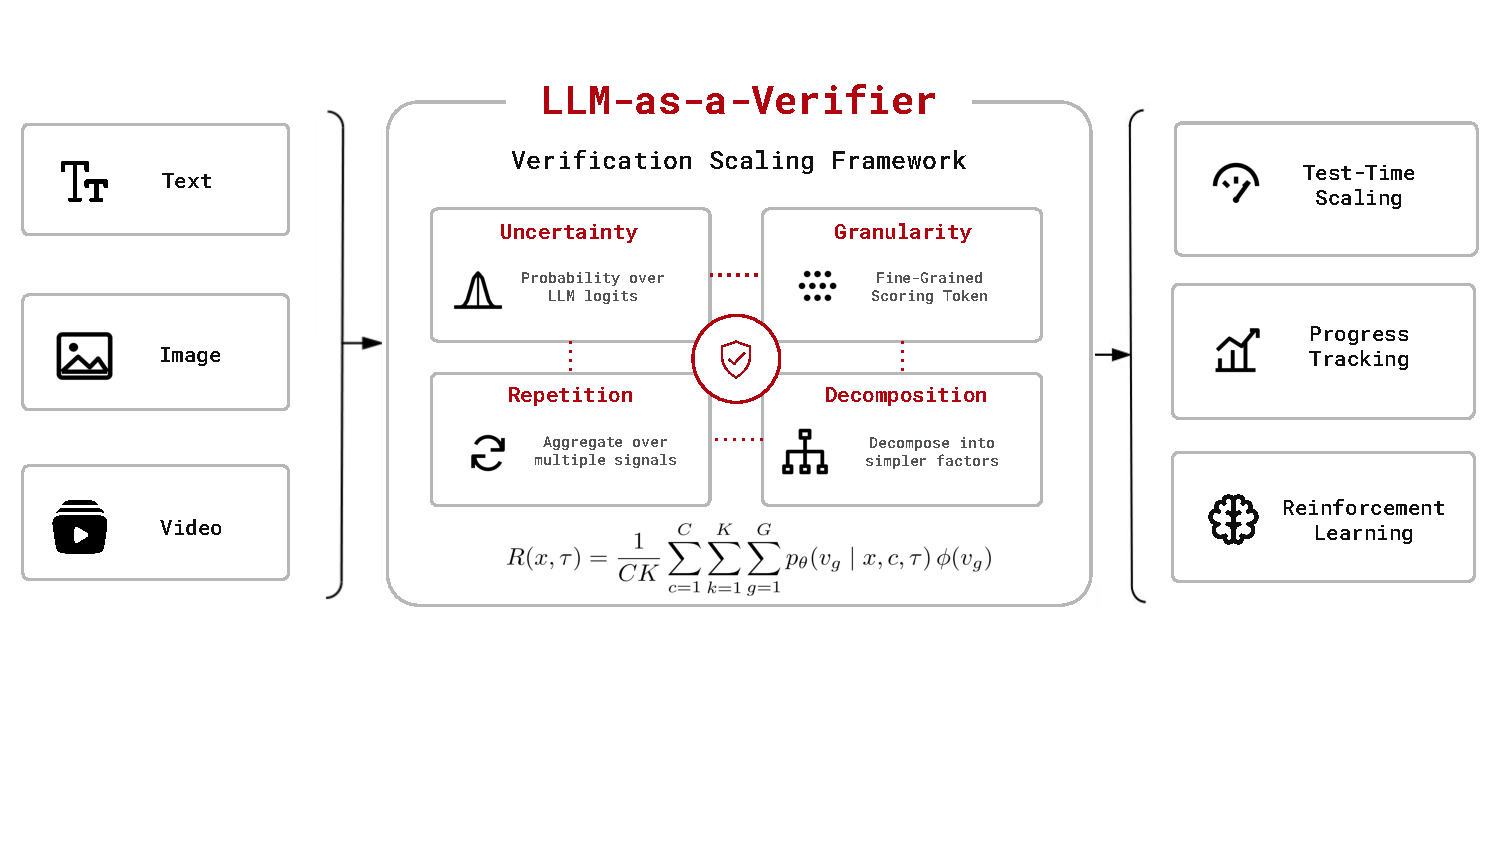
\includegraphics[width=\linewidth]{figures/llmoverview.pdf}
    \caption{\textbf{Multiple modalities, many applications, one unified verification framework.} We present LLM-as-a-Verifier, a general-purpose framework that provides fine-grained feedback for any modality without requiring additional training. By leveraging the full distribution of scoring-token logits, our method captures evaluation uncertainty and enables verification to scale along three dimensions: score granularity, repeated evaluation, and criteria decomposition. The resulting fine-grained feedback can be used for test-time scaling, progress tracking, and reinforcement learning.}
    \label{fig:overview}
\end{figure}

\section{Introduction}
Recent advances in large language models (LLMs) have established scaling as a central paradigm for improving their capabilities. Performance has been driven by scaling along multiple axes, including pre-training data and compute, post-training optimization, and test-time inference~\citep{kaplan_scaling_2020, gao_scaling_2022, snell_scaling_2024}. \begin{wrapfigure}{r}{0.283\textwidth}
    \centering
    \vspace{2pt}
    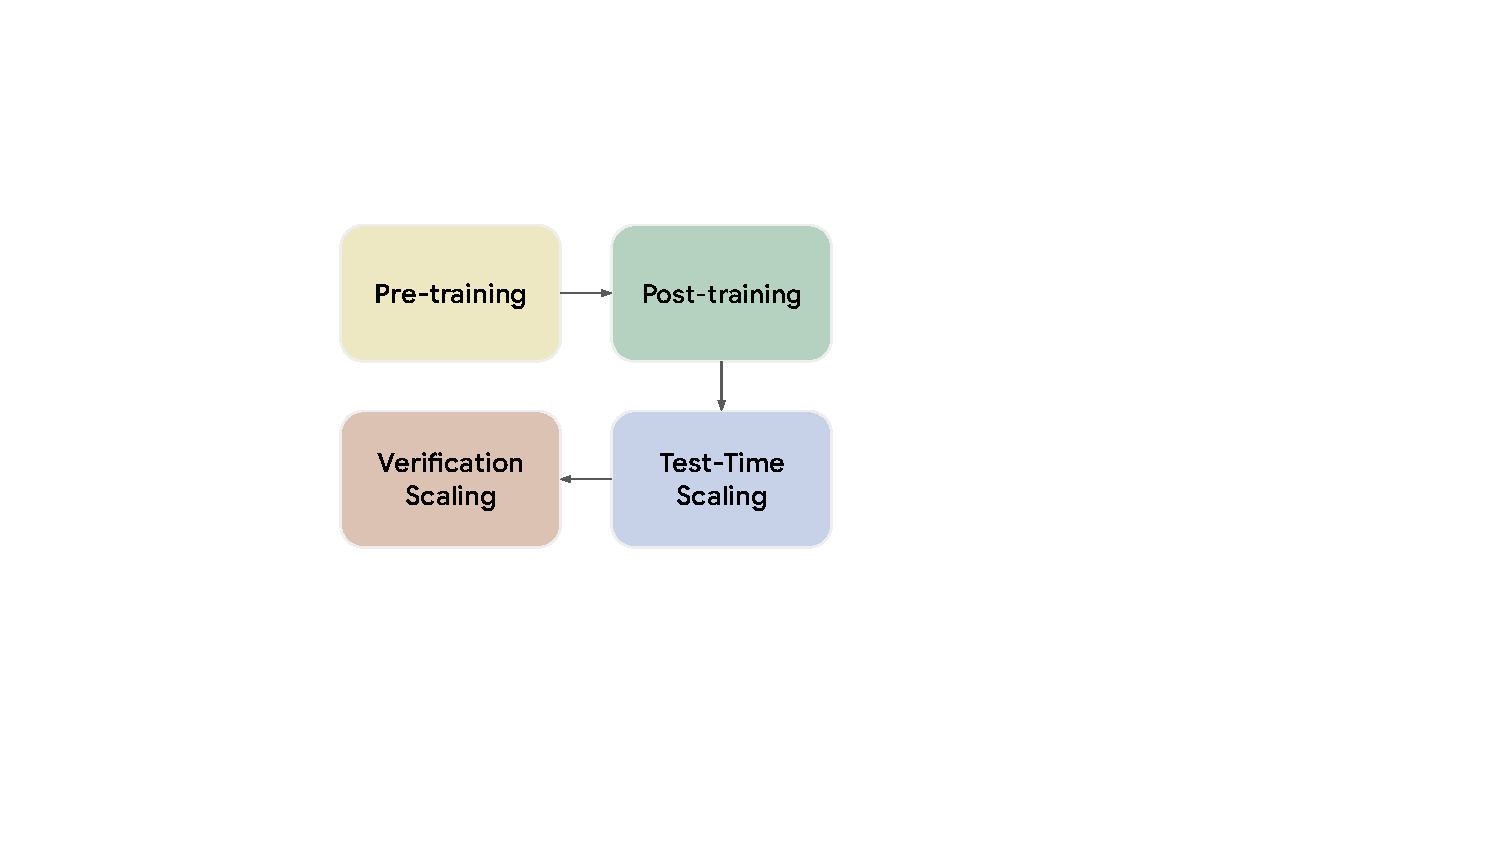
\includegraphics[width=\linewidth]{figures/paradigms.pdf}
    % \vspace{-10pt}
    \caption{Scaling paradigms for large language models.}
    \label{fig:paradigms}
    % \vspace{-10pt}
\end{wrapfigure}However, while generation has benefited significantly from these scaling paradigms, verification---the ability to determine the quality or correctness of a solution---has not seen the same degree of scaling. In this work, we argue that verification itself constitutes a distinct and underexplored scaling axis. Unlike generation, which benefits from well-established scaling laws, verification in current systems remains fundamentally limited. In particular, standard LM judges collapse scoring distributions into coarse discrete scores~\citep{zheng_judging_nodate, singh_v_1_2026}, leading to ties and poor discrimination, while learned reward models are constrained by training data and often fail to generalize across domains~\citep{zhang2025generativeverifiersrewardmodeling, cobbe_training_2021}. These limitations hinder the scalability of verification, preventing further performance improvements.

\begin{figure}[t!]
    \centering
    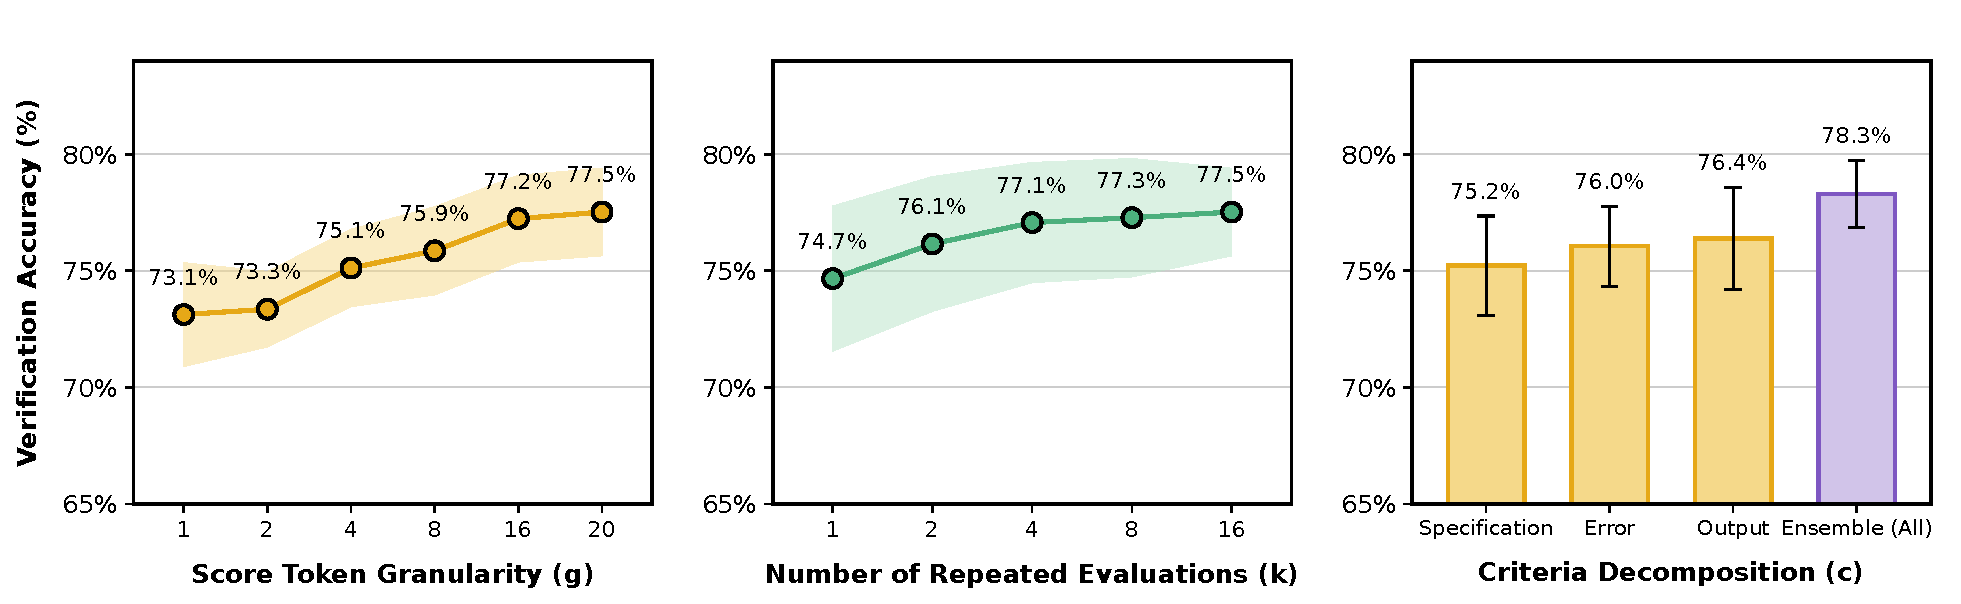
\includegraphics[width=\linewidth]{figures/granularity.pdf}
    \caption{\textbf{Verification Scaling.} We find that verification accuracy consistently improves as we scale across multiple dimensions: (1) the granularity of score tokens, (2) the number of repeated evaluations, and (3) the decomposition of evaluation criteria. Verification accuracy is measured as the pairwise accuracy of the verifier in assigning a higher score to the ground-truth successful solution than to failed solutions for the same task on Terminal-Bench V2.}
    \label{fig:scaling_verifier}
\end{figure}

To this end, we introduce LLM-as-a-Verifier, a general-purpose verification framework that provides dense and fine-grained feedback without requiring additional training. Unlike traditional approaches that prompt LLMs to produce discrete scores within the language space~\citep{zheng_judging_nodate}, LLM-as-a-Verifier estimates the quality of candidate solutions by computing the expectation over the distribution of scoring token logits. In Fig.~\ref{fig:scaling_verifier}, we show that this probabilistic formulation unlocks multiple axes of scaling for verification. We first demonstrate that scaling the number of extracted token logits consistently reduces the tie rate when comparing complex solutions and improves the separation between positive and negative solutions. We observe that an individual evaluation or a single criterion can be biased or noisy. To mitigate this, we scale verification along two additional dimensions, repeated evaluations (which reduces variance) and criteria decomposition (which reduces prompt bias), leading to higher verification accuracy. We quantify these scaling benefits under controlled budgets, comparing LLM-as-a-Verifier against a discrete LM judge baseline in Sec.~\ref{sec:scaling}. To make verification scaling practical, we further introduce a cost-efficient ranking algorithm for selecting the best solution among candidates using the preference probabilities derived from the verifier’s continuous scores.

Interestingly, we find that the fine-grained signals produced by LLM-as-a-Verifier enable the evaluation of entire interaction trajectories rather than only intermediate steps or final outcomes as in PRMs and ORMs~\citep{cobbe_training_2021, lightman_lets_2023} for agentic tasks. When used as a trajectory reward model with our cost-efficient ranking algorithm, LLM-as-a-Verifier outperforms frontier models on challenging benchmarks across coding, robotics, and medical domains. It achieves state-of-the-art performance on Terminal-Bench V2 (86.5\%), SWE-Bench Verified (78.2\%), RoboRewardBench (87.4\% Trajectory Preference Accuracy), and MedAgentBench (73.3\%). 

Beyond its role as a verifier, our approach can also serve as a proxy for estimating task progress. Notably, we observe a strong correlation between the chronological order of steps and the verifier score (Fig.~\ref{fig:voc-counterfactual-code}). To instantiate these capabilities, we provide extensions for Claude Code and Codex, enabling users to monitor task progress and harness the benefits of LLM-as-a-Verifier to improve their own agentic systems. In robotics, our approach outperforms state-of-the-art reward models, including Robometer~\citep{liang2026robometer}, TOPReward~\citep{chen2026topreward}, and RoboReward~\citep{lee2026roboreward}, achieving a mean Value-Order Correlation (VOC) of 0.966. Overall, LLM-as-a-Verifier provides a scalable mechanism for improving the evaluation and monitoring of autonomous agents and robots in real-world environments.

Additionally, we demonstrate that using LLM-as-a-Verifier as a dense reward signal improves the sample efficiency of both off-policy and on-policy reinforcement learning algorithms. On LIBERO~\cite{liu2023liberobenchmarkingknowledgetransfer}, LLM-as-a-Verifier achieves $\approx1.8\times$ higher sample efficiency than sparse reward baselines when fine-tuning a $\pi_0$ policy with DSRL-SAC~\cite{wagenmaker2025steeringdiffusionpolicylatent}, while also reaching a higher final success rate. On the MATH reasoning benchmark, it achieves $\approx1.1\times$ higher sample efficiency when fine-tuning Qwen3-8B with GRPO~\cite{deepseek-ai_deepseek-r1_2025}.
\clearpage

In summary, our contributions are as follows:

\begin{enumerate}
\item We introduce LLM-as-a-Verifier, a probabilistic verification framework that leverages the full distribution of scoring token logits to produce fine-grained feedback and characterize three key axes of verification scaling: (1) score granularity, (2) repeated evaluation, and (3) criteria decomposition.

\item 
We propose a cost-efficient algorithm for ranking candidates and demonstrate that, when combined with verification scaling, LLM-as-a-Verifier achieves state-of-the-art performance across coding, robotics, and medical benchmarks without requiring additional training.

\item
We show that the fine-grained verifier score correlates with an agent's task progress and can be used to monitor the behavior of agents and robots.

\item
We demonstrate that LLM-as-a-Verifier can provide dense feedback for reinforcement learning, improving the sample efficiency of both on-policy and off-policy algorithms across robotics and mathematical reasoning benchmarks.


\end{enumerate}